\section{Performance Modelling}
\label{sec:performance}

We estimate the noise remaining after TDI and clock correction from the measured delay-line noise, the modulation characterization and a prospective optical readout calculation. The calculation uses static delays and ideal cancellation of the common laser and clock noises.

\subsection{Noise Inputs and Comparison Reference}

For laser frequency noise we adopt the LISA pre-stabilization reference \cite{bayle_unified_2023},
\begin{equation}
 A_\nu(f)=30\,\frac{\mathrm{Hz}}{\sqrt{\mathrm{Hz}}}
 \sqrt{1+\left(\frac{2\,\mathrm{mHz}}{f}\right)^4}.
\end{equation}
Its equivalent phase ASD is $A_\phi=A_\nu/(2\pi f)$.

The clock estimate uses the phase-noise model of a 10 MHz Rb standard. Its single-sideband phase noise is anchored at $\mathcal L(10\,\mathrm{Hz})=-130\,\mathrm{dBc/Hz}$, consistent with the specifications in \cite{srs_rb_standard}. Below this point, the phase PSD is extrapolated as $f^{-1}$ down to 1 Hz, $f^{-2}$ down to 10 mHz, and $f^{-3}$ below 10 mHz. The corresponding timing ASD is
\begin{equation}
 A_q(f)=\frac{\sqrt{2\,10^{\mathcal L(f)/10}}}{2\pi\times10\,\mathrm{MHz}}.
\end{equation}
This gives approximately $2.25\,\mathrm{ps}/\sqrt{\mathrm{Hz}}$ at 10 mHz and $71\,\mathrm{ps}/\sqrt{\mathrm{Hz}}$ at 1 mHz. It is an estimate from the assumed low-frequency continuation, rather than a measurement of the laboratory clocks. The common timing noise couples to a carrier link as $|\alpha_{ij}|A_q$ and is removed by the ideal clock correction used here.

The electronic input is the measured delay-line phase-noise floor, including processing and electronics and possibly the readout phasemeter's ADC. The carrier and sideband measurements give the same floor, so we assign the same PSD to each electronic readout term. The terms are taken to be independent between links and channels, while repeated uses of a given readout remain coherent.

The modulation characterization uses half the upper-minus-lower sideband phase of a local optical beat, with a common modulation and measurement reference. The present spectrum is used as an estimate of source modulation phase noise $m_i$. The planned repeat measurement will update this input and test the proposed Moku-generated modulation tone.

Figure~\ref{fig:component_inputs_single_link} shows these component inputs in cycles/$\sqrt{\mathrm{Hz}}$. The measured spectra cover the plotted $0.25\,\mathrm{mHz}$--$1\,\mathrm{Hz}$ band without extrapolation.

For comparison, we use the single-link reference adopted in the component analysis. With $\lambda=1064\,\mathrm{nm}$, its equivalent phase ASDs are
\begin{align}
 A_{\mathrm{OMS}}(f)
 &=\frac{15\times10^{-12}\,\mathrm{m}}{\lambda}
   \sqrt{1+\left(\frac{2\,\mathrm{mHz}}{f}\right)^4},\\
 A_{\mathrm{acc}}(f)
 &=\frac{3\times10^{-15}\,\mathrm{m\,s^{-2}}}{(2\pi f)^2\lambda}
   \sqrt{1+\left(\frac{0.4\,\mathrm{mHz}}{f}\right)^2}\nonumber\\
 &\quad\times
   \sqrt{1+\left(\frac{f}{8\,\mathrm{mHz}}\right)^4}.
\end{align}
The reference is $A_{\mathrm{link}}=(A_{\mathrm{OMS}}^2+A_{\mathrm{acc}}^2)^{1/2}$. Acceleration noise is included here as a comparison quantity; it is not an experimentally present test-mass noise in the current testbed. The component spectra are displayed directly, without applying a TDI transfer function. Consequently, this figure compares input noise scales and does not establish a gravitational-wave sensitivity.

% Two-column-width variant. Use figure, width=\columnwidth, and the
% *_column.pdf filename for a single-column version.
\begin{figure*}[t]
    \centering
    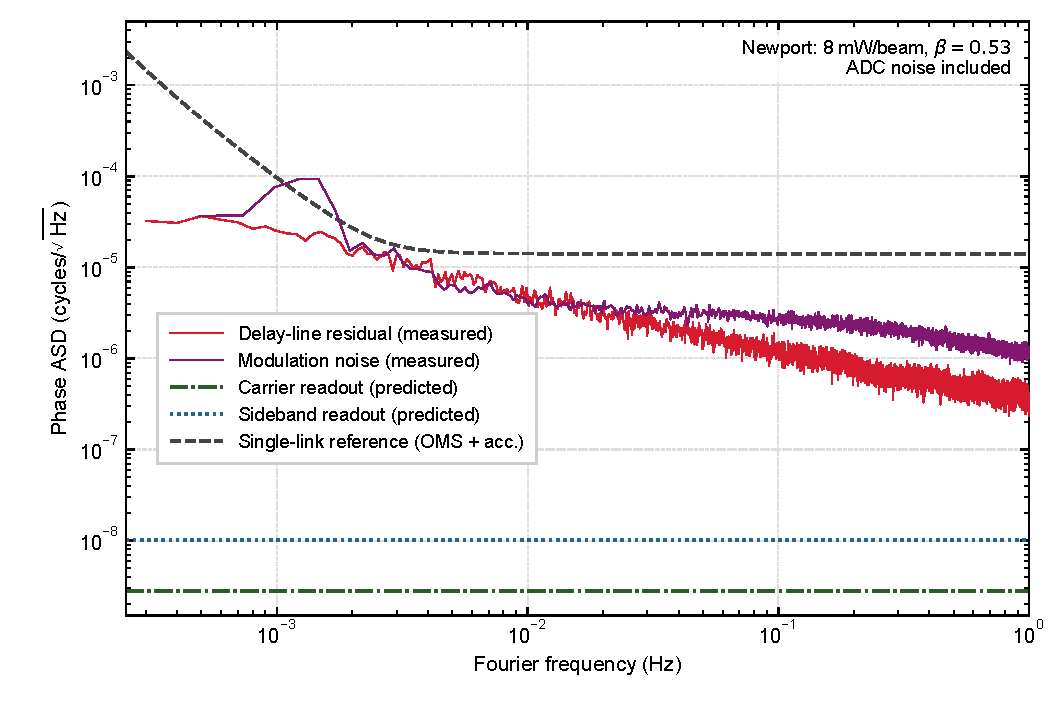
\includegraphics[width=\textwidth]{images/performance/component_inputs_single_link.pdf}
    \caption{Component phase-noise amplitude spectral densities compared with
    the single-link reference formed from optical metrology and acceleration
    noise. Solid curves show the measured delay-line residual and modulation
    phase-noise estimator; measured Fourier bins are plotted without smoothing.
    The illustrative linear-receiver carrier and first-order sideband readout noises
    include shot noise, dark-current shot noise, Johnson noise, relative
    intensity noise and ADC quantization noise. The optical model assumes one
    phase-modulated beam and one unmodulated reference beam, each delivering
    $4\,\mathrm{mW}$ at the detector, with modulation depth $0.53\,\mathrm{rad}$.
    The detector responsivity is $0.6\,\mathrm{A/W}$, heterodyne efficiency is
    $0.9$, and the termination is $50\,\Omega$ at $300\,\mathrm{K}$.
    The ADC model uses a $1\,\mathrm{V}$ full-scale span, 14 bits and
    $2\,\mathrm{GS/s}$, with an ideal three-way electrical split. The assumed white RIN is
    $0.9\times10^{-8}/\sqrt{\mathrm{Hz}}$, summed coherently between the beams.
    The model uses $(35,36,34)\,\mathrm{MHz}$ modulation and electrical carrier
    frequencies of $15.0$, $10.9$ and $21.6\,\mathrm{MHz}$; the readout
    prediction assumes white noise across the corresponding RF bands.
    All curves are shown before propagation through TDI and clock correction;
    the measured electronic residual is shown as characterized and is not
    deconvolved into individual board noise sources. The assumptions of the component budget are stated in Section~\ref{sec:performance}. }
    \label{fig:component_inputs_single_link}
\end{figure*}


\subsection{Predicted Carrier and Sideband Readout Noise}
\label{sec:readout_noise}

For the readout calculation, we consider one phase-modulated laser interfering with an unmodulated reference laser in a prospective Newport PIN-detector readout. Each beam delivers $4\,\mathrm{mW}$ at the detector, after any combining losses, and the phase-modulation depth is $\mu_{\mathrm{EOM}}=0.53\,\mathrm{rad}$. This operating mode provides an explicit carrier--carrier and sideband--carrier readout estimate. The optional configuration with both lasers modulated requires the corresponding sideband--sideband beat amplitudes to be substituted; the present numerical values should not be transferred to that mode without this adjustment.

For optical powers $P_{\mathrm{SC}}$ and $P_{\mathrm{ref}}$, responsivity $\mathcal R$, and power-overlap efficiency $\eta_{\mathrm{het}}$, the peak current of beat order $n$ is
\begin{equation}
 I_{n,\mathrm{pk}}=2\mathcal R
 \sqrt{\eta_{\mathrm{het}}P_{\mathrm{SC}}P_{\mathrm{ref}}}
 \left|J_n(\mu_{\mathrm{EOM}})\right|.
 \label{eq:perf_beat_current}
\end{equation}
The carrier uses $n=0$, and either first-order sideband uses $|n|=1$. Here $J_0(0.53)=0.9310$ and $J_1(0.53)=0.2558$. The modulated beam therefore contains $3.47\,\mathrm{mW}$ in its carrier and $0.262\,\mathrm{mW}$ in each first-order sideband. Using $\mathcal R=0.6\,\mathrm{A/W}$ and $\eta_{\mathrm{het}}=0.9$ gives peak beat currents of $4.24\,\mathrm{mA}$ and $1.16\,\mathrm{mA}$, respectively.

We include shot noise, dark-current shot noise, Johnson noise, relative intensity noise (RIN), and ADC quantization noise. Their one-sided current ASDs are modelled as
\begin{align}
 i_{\mathrm{shot}}&=\sqrt{2e[\mathcal R(P_{\mathrm{SC}}+P_{\mathrm{ref}})+I_d]},\\
 i_{\mathrm J}&=\sqrt{4k_{\mathrm B}T/R_{\mathrm L}},\\
 i_{\mathrm{RIN}}&=\mathcal R(P_{\mathrm{SC}}+P_{\mathrm{ref}})A_{\mathrm{RIN}},\\
 i_{\mathrm{ADC}}&=\frac{V_{\mathrm{FS}}}{2^{B_{\mathrm{ADC}}}G\sqrt{6f_s}}.
\end{align}
The assumed linear-receiver parameters are $I_d=100\,\mathrm{nA}$, $T=300\,\mathrm{K}$, $R_{\mathrm L}=50\,\Omega$, $G=50/\sqrt{3}\,\mathrm{V/A}$, $V_{\mathrm{FS}}=1\,\mathrm V$, $B_{\mathrm{ADC}}=14$ and $f_s=2\,\mathrm{GHz}$. The RIN ASD is $A_{\mathrm{RIN}}=0.9\times10^{-8}/\sqrt{\mathrm{Hz}}$. The RIN expression retains a conservative coherent sum of the two beams' intensity fluctuations. It represents additive noise around the RF beat frequencies; low-frequency amplitude modulation is not assumed to couple directly to phase. The ADC term uses the physical conversion rate $f_s=2\,\mathrm{GS/s}$, before the 125 MHz FPGA processing described in Section~\ref{sec:delay_line}. It assumes white quantization noise and appropriate antialias filtering; a decimated output rate is not a substitute for $f_s$ in this estimate.

The gain assumes a $50\,\mathrm{V/A}$ detector output followed by an ideal matched three-way electrical split. The split attenuates the signal and detector noise equally, while increasing the input-referred ADC contribution. At $4\,\mathrm{mW}$ per beam, the mean and maximum instantaneous optical powers are $8$ and $15.6\,\mathrm{mW}$, respectively, below the detector's listed $20\,\mathrm{mW}$ maximum \cite{newport1064}. After DC removal, the ideal phase-modulated beat has a peak-to-peak voltage of approximately $0.263\,\mathrm V$ at each ADC. These assumptions provide headroom for the prospective readout; additional RF losses are not included.

For additive noise that is locally white around the selected beat, demodulation combines noise from both RF sidebands. The equivalent phase ASD of contribution $k$ is
\begin{equation}
 A_{\phi,n}^{(k)}=\frac{\sqrt{2}\,i_k}{2\pi I_{n,\mathrm{pk}}}.
 \label{eq:perf_phase_asd}
\end{equation}
The factor $2\pi$ converts radians to cycles. No integration over the PLL bandwidth is applied to these spectral densities. Summing the component PSDs gives carrier and first-sideband readout ASDs of $3.40\times10^{-9}$ and $1.24\times10^{-8}$ cycles/$\sqrt{\mathrm{Hz}}$, respectively, equivalent to $21.4$ and $77.8\,\mathrm{nrad}/\sqrt{\mathrm{Hz}}$. Their ratio is $J_0(\mu_{\mathrm{EOM}})/|J_1(\mu_{\mathrm{EOM}})|\simeq3.64$. These are predictions for the stated optical powers and white-noise assumptions, not measurements of the complete readout chain.

\begin{figure*}[t]
 \centering
 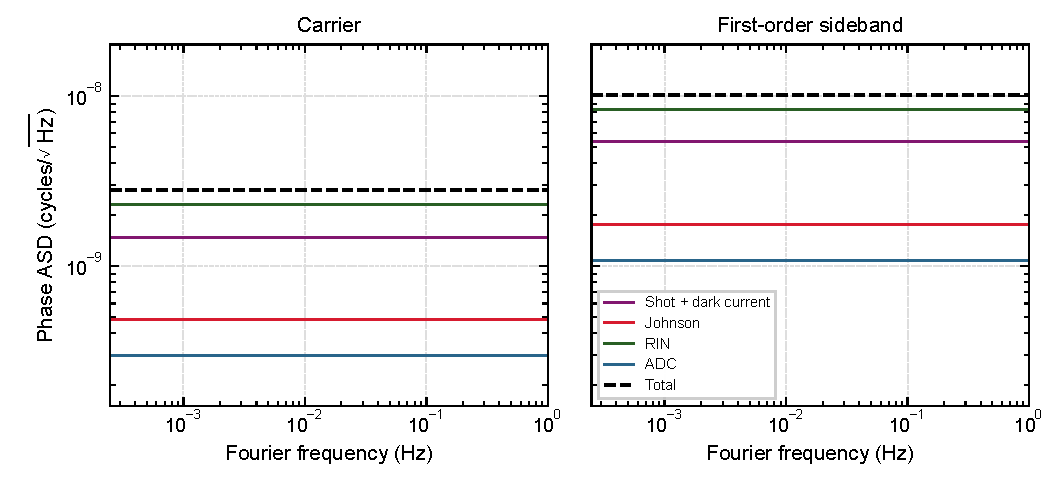
\includegraphics[width=\textwidth]{images/performance/newport_readout_breakdown.pdf}
 \caption{Illustrative linear-receiver carrier and first-order sideband readout noise for one modulated and one unmodulated beam, each delivering $4\,\mathrm{mW}$ at the detector, with modulation depth $0.53\,\mathrm{rad}$. The two panels share a common vertical scale. Shot noise includes dark-current shot noise; the ADC contribution is the white quantization estimate. The dashed curves are the quadrature totals. The beat amplitudes in Eq.~\eqref{eq:perf_beat_current} set the different phase-noise levels. The ADC estimate includes an ideal three-way electrical split.}
 \label{fig:newport_readout}
\end{figure*}

The signal levels explain why this readout operates differently from LISA's. The $4\,\mathrm{mW}$ laboratory beams produce strong carrier and sideband beats, whereas LISA must measure light received after propagation over millions of kilometres. miniLISA therefore has a much lower predicted detector readout noise than the LISA science-interferometer allocations, as summarized in Table~\ref{tab:noise_comparison}.

The testbed does not need to reproduce LISA's weak-light, shot-noise-limited readout to test laser- and clock-noise suppression. A lower readout floor makes smaller residuals from the delay and clock-transfer chains accessible. Shot noise is included in the calculation. The measured electronic residual and sideband-difference estimator exceed the calculated input readout noise; their contributions to the corrected observable depend on the source propagation discussed below. Thus the laboratory signal powers are chosen to support the noise-suppression tests, rather than to reproduce the mission's photon budget.

The LISA allocations (IRD2--IDS--04010 and IRD2--IDS--04580) increase towards low frequencies as $\sqrt{1+(f_k/f)^4}$, with $f_k=2\,\mathrm{mHz}$ for the carrier and $0.7\,\mathrm{mHz}$ for the sidebands. They refer to individual readouts and are distinct from the total OMS-plus-acceleration comparison curve used above.

These input noise levels do not by themselves specify the output noise after TDI. In particular, detector noise shared by the split input paths and noise added independently by each board have different transfer functions.

\subsection{Propagation Through TDI and Clock Correction}
\label{sec:noise_propagation}

The propagation calculation uses the four links of Michelson $X$, static delays and constant nominal frequencies. The illustrative frequency plan is $\nu_{\mathrm R,i}=(15.0,10.9,21.6)\,\mathrm{MHz}$ and $\nu_i^m=(35,36,34)\,\mathrm{MHz}$, giving $(\alpha_{12},\alpha_{21},\alpha_{13},\alpha_{31})=(-4.1,4.1,6.6,-6.6)\,\mathrm{MHz}$. The nominal one-way delay is $L=2.5\times10^9\,\mathrm m/c\simeq8.339\,\mathrm s$. These are example operating frequencies. The small modulation-frequency offsets separate the synthesized carrier and sideband beats; the laboratory readout is not constrained to the representative LISA 5--25 MHz band.
Writing $z_{ij}=\exp(-2\pi\mathrm i f d_{ij})$, $A=z_{12}z_{21}$ and $B=z_{13}z_{31}$, the static Michelson defined above becomes
\begin{align}
 X={}&(1-A)(\eta_{13}+z_{13}\eta_{31})\nonumber\\
     &-(1-B)(\eta_{12}+z_{12}\eta_{21}).
\end{align}
Let $P_{ij}$ denote its four link coefficients and $K_{ij}$ the clock-correction coefficients, chosen so that
\begin{equation}
 X_{\mathrm c}=\sum_{ij}(P_{ij}\eta_{ij}+K_{ij}r_{ij})
\end{equation}
has zero coefficient for each $q_i$. The sum runs over links $12$, $21$, $13$ and $31$, using the upper-sideband-minus-carrier definition of $r_{ij}$ given above. The static second-generation convention used in the calculation is $X_{2\mathrm c}=(1-AB)X_{\mathrm c}$; this extra filter must multiply both the science and correction weights. Laser and clock cancellation can be checked algebraically for unequal static delays. The calculation is restricted to static arms.

For four independent link noises with the same ASD $A_e$, the uncorrected TDI output is
\begin{equation}
 A_{X,e}=A_e\sqrt{\sum_{ij}|P_{ij}|^2}.
\end{equation}
Four unit-weight terms would give $\sqrt{4}A_e=2A_e$. TDI also contains delayed differences, so its weights depend on Fourier frequency. For equal delays $d$, the static $X_2=(1-AB)X$ convention gives $A_{X_2,e}=8|\sin(2\pi fd)\sin(4\pi fd)|A_e$ before clock correction.

For noise added to individual links, repeated appearances of one readout must be combined coherently. In particular, for the first-generation weights the coefficients are
\begin{equation}
 T_{b^{\mathrm c}_{ij}}=P_{ij}-\frac{K_{ij}}{\nu_j^m},\qquad
 T_{b^{\mathrm{sb,+}}_{ij}}=\frac{K_{ij}}{\nu_j^m}.
\end{equation}
The two appearances of a given carrier noise are therefore combined before taking a squared magnitude. These coefficients apply directly to $e^a_{ij}$ in Eq.~\eqref{eq:shared_readout}, not to independent copies of a shared detector noise.

For matched paths, the shared carrier term $\mathbf D_{ij}p_j^{\mathrm c}-p_i^{\mathrm c}$ has the laser-noise structure and cancels in carrier TDI. However, define the detector channel difference $\chi_i=p_i^{\mathrm{sb,+}}-p_i^{\mathrm c}$. It contributes to the clock-transfer variable as
\begin{equation}
 r_{ij}^{\mathrm{det}}=\frac{z_{ij}\chi_j-\chi_i}{\nu_j^m},
\end{equation}
and hence to the corrected observable as
\begin{equation}
 X_{2\mathrm c}^{\mathrm{det}}=(1-AB)\sum_{ij}K_{ij}
 \frac{z_{ij}\chi_j-\chi_i}{\nu_j^m}.
 \label{eq:detector_clock_residual}
\end{equation}
For the estimate, detector noise in the carrier and sideband channels is taken to be independent, so $S_{\chi_i}=S_{p_i^{\mathrm{sb,+}}}+S_{p_i^{\mathrm c}}$. Copies of each detector channel shared between boards retain the same noise realization.

 For independent physical sources $n_a$, the output PSD is
\begin{equation}
 S_{X_{2\mathrm c}}(f)=\sum_a|T_a(f)|^2 S_a(f).
\end{equation}
The measured electronic spectrum is propagated with the carrier and sideband coefficients above. The predicted detector terms use Eq.~\eqref{eq:detector_clock_residual}. ADC quantization is shown in the input readout estimate but is not added separately to the total, where electronics are represented by the measured delay-line floor.

True source modulation noise survives clock correction. At fixed nominal beat frequencies, increasing all $\nu_i^m$ by a common factor $s$ reduces its transfer coefficients by $1/s$. The output modulation ASD therefore decreases by $1/s$ for fixed direct phase noise. For fixed timing noise, the input modulation phase ASD increases by $s$, leaving the residual unchanged. These scaling statements apply to the identified physical source, not automatically to the full measured sideband-difference spectrum. Likewise, a small raw TDI ASD at low Fourier frequency partly reflects the differencing response of the observable, which also acts on a gravitational-wave signal; it is not by itself an improvement in sensitivity.

\subsection{Estimated Residual Noise}

Figure~\ref{fig:total_tdi2_noise} combines the electronic, modulation and detector contributions after static second-generation TDI and clock correction. Each physical source is multiplied by its transfer function before the output PSDs are summed. The calculation uses four independent electronic link readouts per channel and three shared detector inputs, with the assumptions given above. The detector contribution is small compared with the measured electronic and modulation inputs, consistent with the use of bright laboratory beams rather than a weak-light readout.

\begin{figure*}[t]
 \centering
 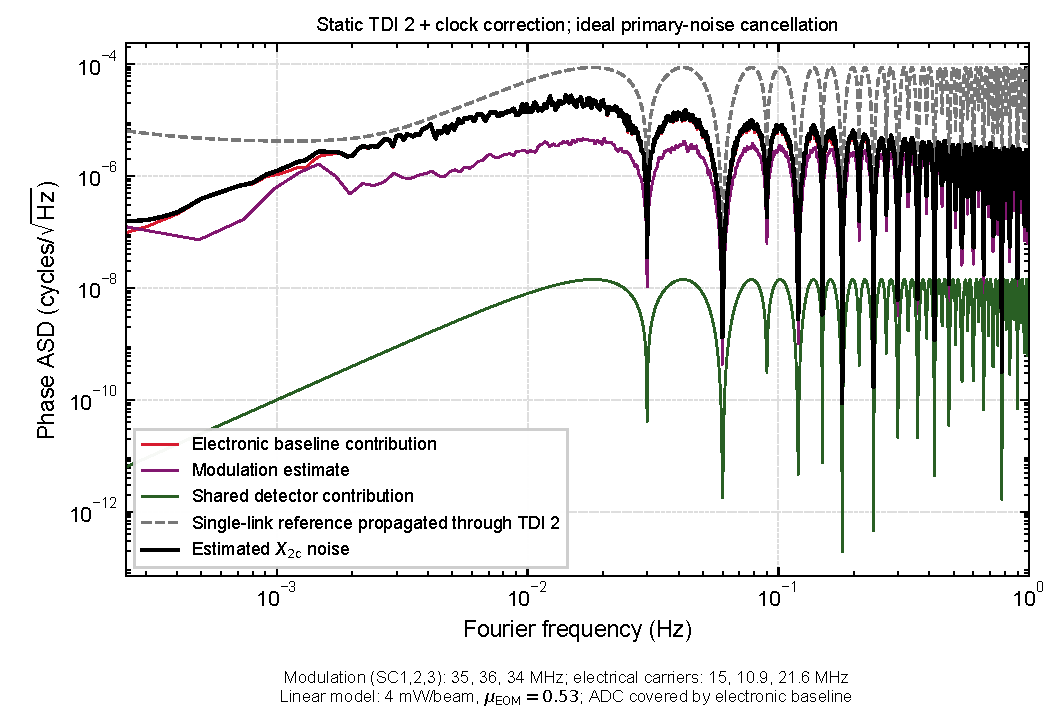
\includegraphics[width=\textwidth]{images/performance/total_noise_tdi2_corrected_budget.pdf}
 \caption{Estimated phase-noise ASD of the clock-corrected static Michelson observable $X_{2\mathrm c}$. The black curve sums the electronic, modulation and shared-detector contributions in quadrature. The calculation uses four links with $8.339\,\mathrm s$ delays, modulation frequencies $(35,36,34)\,\mathrm{MHz}$, and the optical operating point of Section~\ref{sec:readout_noise}. ADC noise is represented by the measured electronic baseline. The dashed comparison curve treats the single-link OMS-plus-acceleration reference as independent equivalent link noises propagated through the same TDI observable. Laser and common clock noise cancel ideally in this static estimate.}
 \label{fig:total_tdi2_noise}
\end{figure*}

The estimate uses the current modulation spectrum, which will be replaced after the planned repeat measurement. It describes the included component noises under ideal primary-noise cancellation, rather than a measured sensitivity of the assembled optical testbed.

Board timing also changes the physical delay, even when the programmed delay is known exactly. For constant $d_{ij}$, Eq.~\eqref{eq:board_delay_jitter} gives
\begin{equation}
 A_{\delta d^\epsilon_{ij}}(f)
 =2|\sin(\pi f d_{ij})|A_{\epsilon_i}(f).
\end{equation}
The common board timing cancels in the linear model discussed above; differential timing can remain. Its nominal beat-frequency coupling is already included in the $\epsilon_i$ terms and is not a separate independent ranging noise. No additional timing or delay-error floor is assigned in the present estimate.

Under the common carrier/sideband GW approximation, the injected signal in this static observable is
\begin{equation}
 X_{2\mathrm c}^{\mathrm{GW}}=(1-AB)\sum_{ij}P_{ij}\delta\phi^{\mathrm{GW}}_{ij}.
\end{equation}
This provides the amplitude and phase prediction for a subsequent hardware injection test.
